\section{Phase-Decomposed Renewal Drift}

The renewal-scale drift data have a compatible phase interpretation.  Split
accelerated steps by the pre-step odd integer modulo \(4\): \(n\equiv 3
\pmod 4\), equivalently \(\vTwo(n+1)\geq 2\), is tail-internal and has forced
valuation \(a=1\); \(n\equiv 1\pmod 4\) is the post-exit phase
\(\artifact{renewal_drift_phase_decomposed.json}{renewal\_drift\_phase\_decomposed.json}\).
The asymptotic post-exit valuation target in this convention is \(3\), not
\(2\): it is the shifted-Geometric value seen after removing the deterministic
tail-internal valuation-one steps.

The symbolic mean-step identity suggested by the artifacts is
\[
  \mu_{\mathrm{step}}
    = \frac12\log_2(3/2)+\frac12\log_2(3/4)
    = \log_2(3/4),
\]
with \(E[a\mid\text{tail}]=1\) and asymptotic
\(E[a\mid\text{post-exit}]=3\)
\(\artifact{renewal_drift_per_step.json}{renewal\_drift\_per\_step.json}\),
\(\artifact{renewal_drift_phase_decomposed.json}{renewal\_drift\_phase\_decomposed.json}\),
\(\artifact{renewal_drift_phase_decomposed_n0_stability.json}{renewal\_drift\_phase\_decomposed\_n0\_stability.json}\).

Across \([10^2,10^4]\) through \([10^{12},10^{15}]\), the post-exit valuation
deviation shrinks from \(-0.03473021694546086\) to
\(-0.006503489706314536\), with monotone absolute decrease and log10-slope
\(-0.06656531395656089\) per decade.  From the \([10^6,10^9]\) window onward,
the total drift deviation is below \(0.01\), ending in the \(0.005\) range.
It is not strictly monotone at the deepest window, moving from
\(0.005160187031614694\) to \(0.0054062766596057465\), a change smaller than
the reported deepest-window CI halfwidth \(0.0005710918683108357\)
\(\artifact{renewal_drift_phase_decomposed_n0_stability.json}{renewal\_drift\_phase\_decomposed\_n0\_stability.json}\).
The saved verdict is \(\texttt{non\_monotone\_or\_flat}\).

\begin{figure}
  \centering
  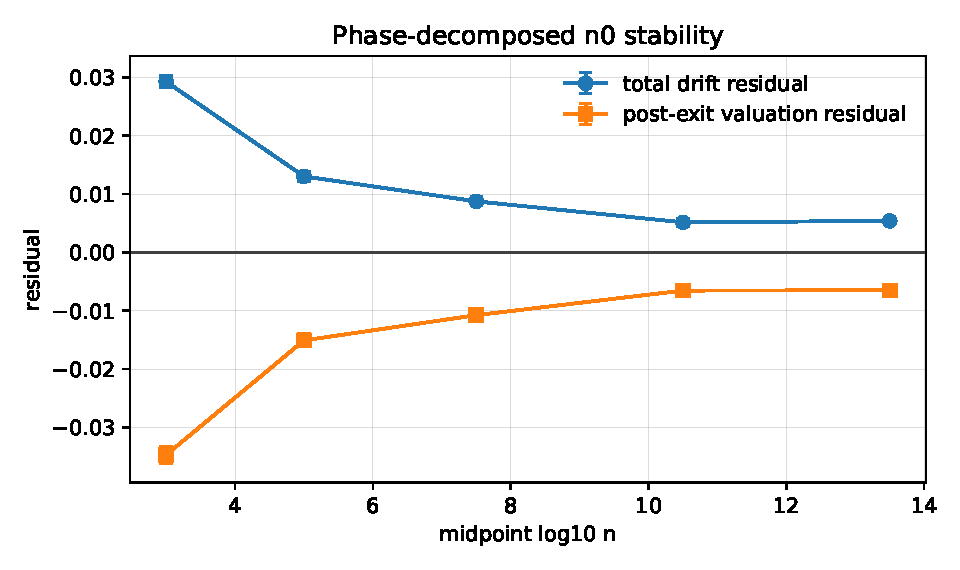
\includegraphics[width=0.86\linewidth]{figures/drift_residual_n0.pdf}
  \caption{Finite-window residuals from the phase-decomposed renewal audit,
  regenerated from
  \artifact{renewal_drift_phase_decomposed_n0_stability.json}{renewal\_drift\_phase\_decomposed\_n0\_stability.json}.}
  \label{fig:drift-residual}
\end{figure}

The caveat is essential.  These artifacts combine a finite audit of bounded
simple cycles on finite LTE-closed tail graphs with finite-window empirical
renewal drift estimates.  They do not prove a global per-orbit Lyapunov
function, do not control arbitrary infinite switching paths, and do not imply a
Collatz descent theorem.
